\documentclass[11pt]{scrartcl}

\usepackage[sexy]{evan}
\usepackage{pgfplots}
\pgfplotsset{compat=1.15}
\usepackage{mathrsfs}
\usetikzlibrary{arrows}
\usepackage{graphics}
\usepackage{tikz}
\usepackage{ amssymb }
\usepackage[dvipsnames]{xcolor}
\usepackage[utf8]{inputenc}
\usepackage{longtable}
\usepackage{ragged2e}
\usepackage{listings}


\definecolor{noseve}{RGB}{242,242,242}

\newcommand{\camod}[1]{\frac{\ZZ}{#1 \ZZ}}
\newcommand{\modm}[1]{\text{ mod } #1}
\newcommand{\campm}[1]{\frac{\ZZ}{m\ZZ}}

\usepackage{epigraph}
\renewcommand{\epigraphsize}{\scriptsize}
\renewcommand{\epigraphwidth}{60ex}


\definecolor{dcol0}{HTML}{C8E6C9}
\definecolor{dcol1}{HTML}{D4E9B3}
\definecolor{dcol2}{HTML}{E5ED9A}
\definecolor{dcol3}{HTML}{FFF59D}
\definecolor{dcol4}{HTML}{FFE082}
\definecolor{dcol5}{HTML}{FFCC80}
\definecolor{dcol6}{HTML}{FFAB91}
\definecolor{dcol7}{HTML}{F49890}
\definecolor{dcol8}{HTML}{E57373}
\definecolor{dcol9}{HTML}{D32F2F}

\makeatletter
\newcommand{\getcolorname}[1]{dcol#1}
\makeatother

\newcommand{\dif}[1]{%
    \edef\colorindex{\number\fpeval{floor(#1)}}%
    \edef\fulltext{#1}%
    \colorbox{\getcolorname{\colorindex}}{%
        \ifnum\colorindex>8
            \textbf{\textcolor{white}{\,\fulltext\,}}%
        \else
            \textbf{\textcolor{black}{\,\fulltext\,}}%
        \fi
    }%
}
% Variable para dificultad (inicial 0)
\newcommand{\thmdifficulty}{0}

% Comando para asignar dificultad antes del problema
\newcommand{\problemdiff}[1]{\renewcommand{\thmdifficulty}{#1}}

% Estilo del problema que incluye dificultad antes del título
\declaretheoremstyle[
    headfont=\color{blue!40!black}\normalfont\bfseries,
    headformat={%
      \dif{\thmdifficulty}\quad \NAME~\NUMBER\ifx\relax\EMPTY\relax\else\ \NOTE\fi
    },
    postheadspace=1em,
    spaceabove=8pt,
    spacebelow=8pt,
    bodyfont=\normalfont
]{problemstyle}

    \declaretheorem[style=problemstyle,name=Problema,sibling=theorem]{problema}
    \declaretheorem[style=problemstyle,name=Problema,numbered=no]{problema*}

%\usepackage[
%backend=biber,
%style=alphabetic,
%sorting=ynt
%]{biblatex}
%\addbibresource{referencias.bib}

\newcommand{\indicacion}[1]{\noindent\textit{\small #1}}


\title {Practica 4: Termistor}
\subtitle{Sistemas de Medicion y Control 18MPEDS0730 \\ Ago-Dic 2025 \\ Centro de Enseñanza Tecnica Industrial Plantel Colomos\\Tgo. en Desarrollo de Software \\ Academia: Sistemas Electrónicos\\Profesor: Diana Marisol Figueroa Flores }
\date{9 de octubre de 2025}
\author{Emmanuel Buenrostro 22300891 7F1 \\ \and Emiliano Arzate 22300929 7F1 \\}


\begin{document}

\maketitle
\begin{center}
   
\includegraphics[scale=0.15]{../../cetilogo.jpg} 
\end{center}
\newpage

\section{Competencias}
\textbf{Competencia a la que aporta al perfil de egreso: }
Integra los conocimientos de la electrónica analógica, digital, sensores y transductores para el desarrollo de aplicaciones de control de lazo abierto y lazo cerrado

\section{Objetivo}

\textbf{Objetivo General:}
Experimentar el funcionamiento de un termistor.
\\


\textbf{Objetivos Específicos:} 
Verificar el funcionamiento básico de un termistor de coeficiente positivo, utilizando un acondicionamiento tipo puente para mandar la señal hacia un sistema de adquisición de datos.


\section{Desarrollo Teórico}

\subsection{Resumen }

\indicacion{
  Elaborar un resumen sobre los diferentes tipos de termistores. Anexar las referencias bibliográficas una referencia deberá ser virtual y la otra de un libro, considerando el formato APA correspondiente al tipo de referencia.
}

\subsection{Material}

\indicacion{
Anotar el material y equipo para llevar a cabo la práctica agregando los valores teóricos.}

\subsection{Caracteristicas Electricas de los Componentes}
\indicacion{
   Anexar características eléctricas de todos los componentes a utilizar, así como los voltajes y corrientes máximas de trabajo, distribución de terminales, etc.
}




\subsection{Diagrama a Bloques}

\begin{center}
    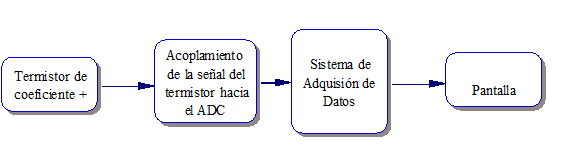
\includegraphics{DiagramaBloques.png}
\end{center}


\subsection{Calculos}
\indicacion{
Realizar los cálculos correspondientes para el acoplamiento de la señal del termistor hacia la entrada analógica del sistema de adquisición de datos.
}


\subsection{Tabla de Valores Teoricos de circuito emisor común con CD}
\indicacion{
Agregar la tabla de valores teóricos de circuito emisor común con divisor de voltaje del amplificador por divisor de voltaje en corriente directa
}

\section{Desarrollo Practico}

\subsection{Pasos}
\indicacion{
    Describe los pasos desde el inicio de la elaboración de la práctica hasta el término de la misma
}

\subsection{Diagrama Electrico}
\indicacion{
    Dibujar el Diagrama eléctrico utilizando algún programa para elaborar circuitos electrónicos, sin olvidar el valor de los componentes reales.
}

\subsection{Programa}

\indicacion{
    Anexa el programa utilizado para la realización de tu práctica.
}


\subsection{Valores Prácticos}
\begin{center}
\begin{tabular}{|p{4cm}|p{4cm}|p{4cm}|p{4cm}|}
\hline
\textbf{Resistencia medida del termistor}& \textbf{Voltaje de Acoplamiento} & \textbf{Voltaje entrada Analógica en Binario} & \textbf{Valor que se muestra Decimal}\\
\hline
6.75k & 1.871V& 01000000 &64 \\[4px]
\hline
7.27k & 2V & 01101010& 102 \\[4px]
\hline
8k &2.1v & &111 \\[4px]
\hline
9.1k& 2.18V&01110011 &115 \\[4px]
\hline
13.8K& 2.3V& 01110111& 119\\[4px]
\hline
15K& 2.37& 01111001 & 121 \\[4px]
\hline
19K& 2.45V& & 125 \\[4px]
\hline
21.5K& 2.53& &129 \\[4px]
\hline
38.8K& 2.56V& & 131\\[4px]
\hline
64.6K& 2.64V& & 135\\[4px]
\hline
\end{tabular}
\end{center}


\textbf{Gráfica de Respuesta del Termistor}
\begin{center}
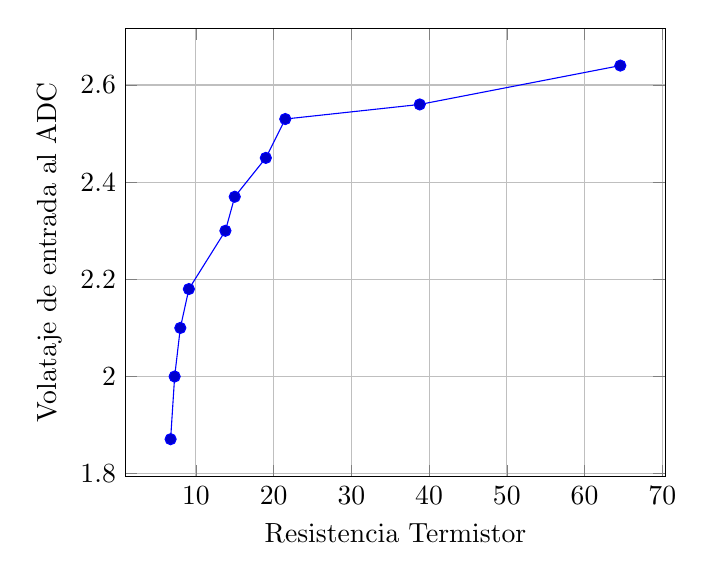
\begin{tikzpicture}
    \begin{axis}[
        ylabel={Volataje de entrada al ADC},
        xlabel={Resistencia Termistor},
        grid=major
    ]
        \addplot coordinates {(6.75,1.871) (7.27,2) (8,2.1) (9.1,2.18) (13.8,2.3) (15,2.37) (19,2.45) (21.5,2.53) (38.8,2.56) (64.6,2.64) };
    \end{axis}
\end{tikzpicture}
 \end{center}



\section{Observaciones y Conclusiones}

\subsection{Observaciones}
\indicacion{
    Elaborar las observaciones correspondientes.
}

\subsection{Conclusiones Personales}
\indicacion{
    Realizar las conclusiones correspondientes de forma personal anexando usos y aplicaciones de lo aprendido.
}


  
%\nocite{*}

%\printbibliography[
%heading=bibintoc,
%title={ . }
%]
    \end{document}